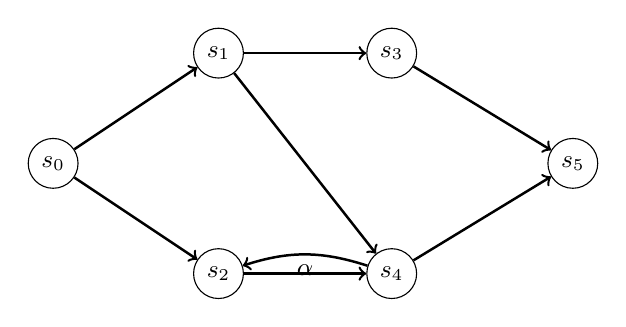
\begin{tikzpicture}[
  scale=1.0,
  state/.style={circle, draw=black, minimum size=18pt, inner sep=0pt},
  every node/.style={font=\small}
]
  \node[state] (s0) at (0.0, 0.0) {\(s_0\)};
  \node[state] (s1) at (2.1, 1.4) {\(s_1\)};
  \node[state] (s2) at (2.1,-1.4) {\(s_2\)};
  \node[state] (s3) at (4.3, 1.4) {\(s_3\)};
  \node[state] (s4) at (4.3,-1.4) {\(s_4\)};
  \node[state] (s5) at (6.6, 0.0) {\(s_5\)};

  \draw[->, line width=0.9pt] (s0) -- (s1);
  \draw[->, line width=0.9pt] (s0) -- (s2);
  \draw[->, line width=0.9pt] (s1) -- (s3);
  \draw[->, line width=0.9pt] (s1) -- (s4);
  \draw[->, line width=0.9pt] (s2) -- (s4);
  \draw[->, line width=0.9pt] (s3) -- (s5);
  \draw[->, line width=0.9pt] (s4) -- (s5);
  \draw[->, line width=0.9pt] (s4) to[bend right=18] node[below] {\(\alpha\)} (s2);
\end{tikzpicture}
